% QumirDB architecture cheat sheet.
%
% Build:  latexmk -pdf architecture.tex
% or:     pdflatex architecture.tex
%
% Keep this in sync with the prose in docs/arch/README.md.

\documentclass[border=14pt]{standalone}

\usepackage[T1]{fontenc}
\usepackage{tikz}
\usetikzlibrary{arrows.meta,positioning,fit,backgrounds}

\definecolor{planfill}{HTML}{DCE9F5}
\definecolor{plandraw}{HTML}{2F6F9F}
\definecolor{kernelfill}{HTML}{E3F0DE}
\definecolor{kerneldraw}{HTML}{4C8C3F}
\definecolor{udffill}{HTML}{FBEFD6}
\definecolor{udfdraw}{HTML}{B5871F}
\definecolor{runfill}{HTML}{EDE3F2}
\definecolor{rundraw}{HTML}{7A57A0}
\definecolor{bandfill}{HTML}{F7F7F7}
\definecolor{banddraw}{HTML}{D0D0D0}
\definecolor{muted}{HTML}{8A8A8A}

% Second line inside a box: the approach or the qualifier, not a repeat.
\newcommand{\sub}[1]{\\[0.6mm]{\footnotesize\color{black!55}#1}}

\begin{document}
% Coordinates are millimetres; lengths inside styles carry their own units.
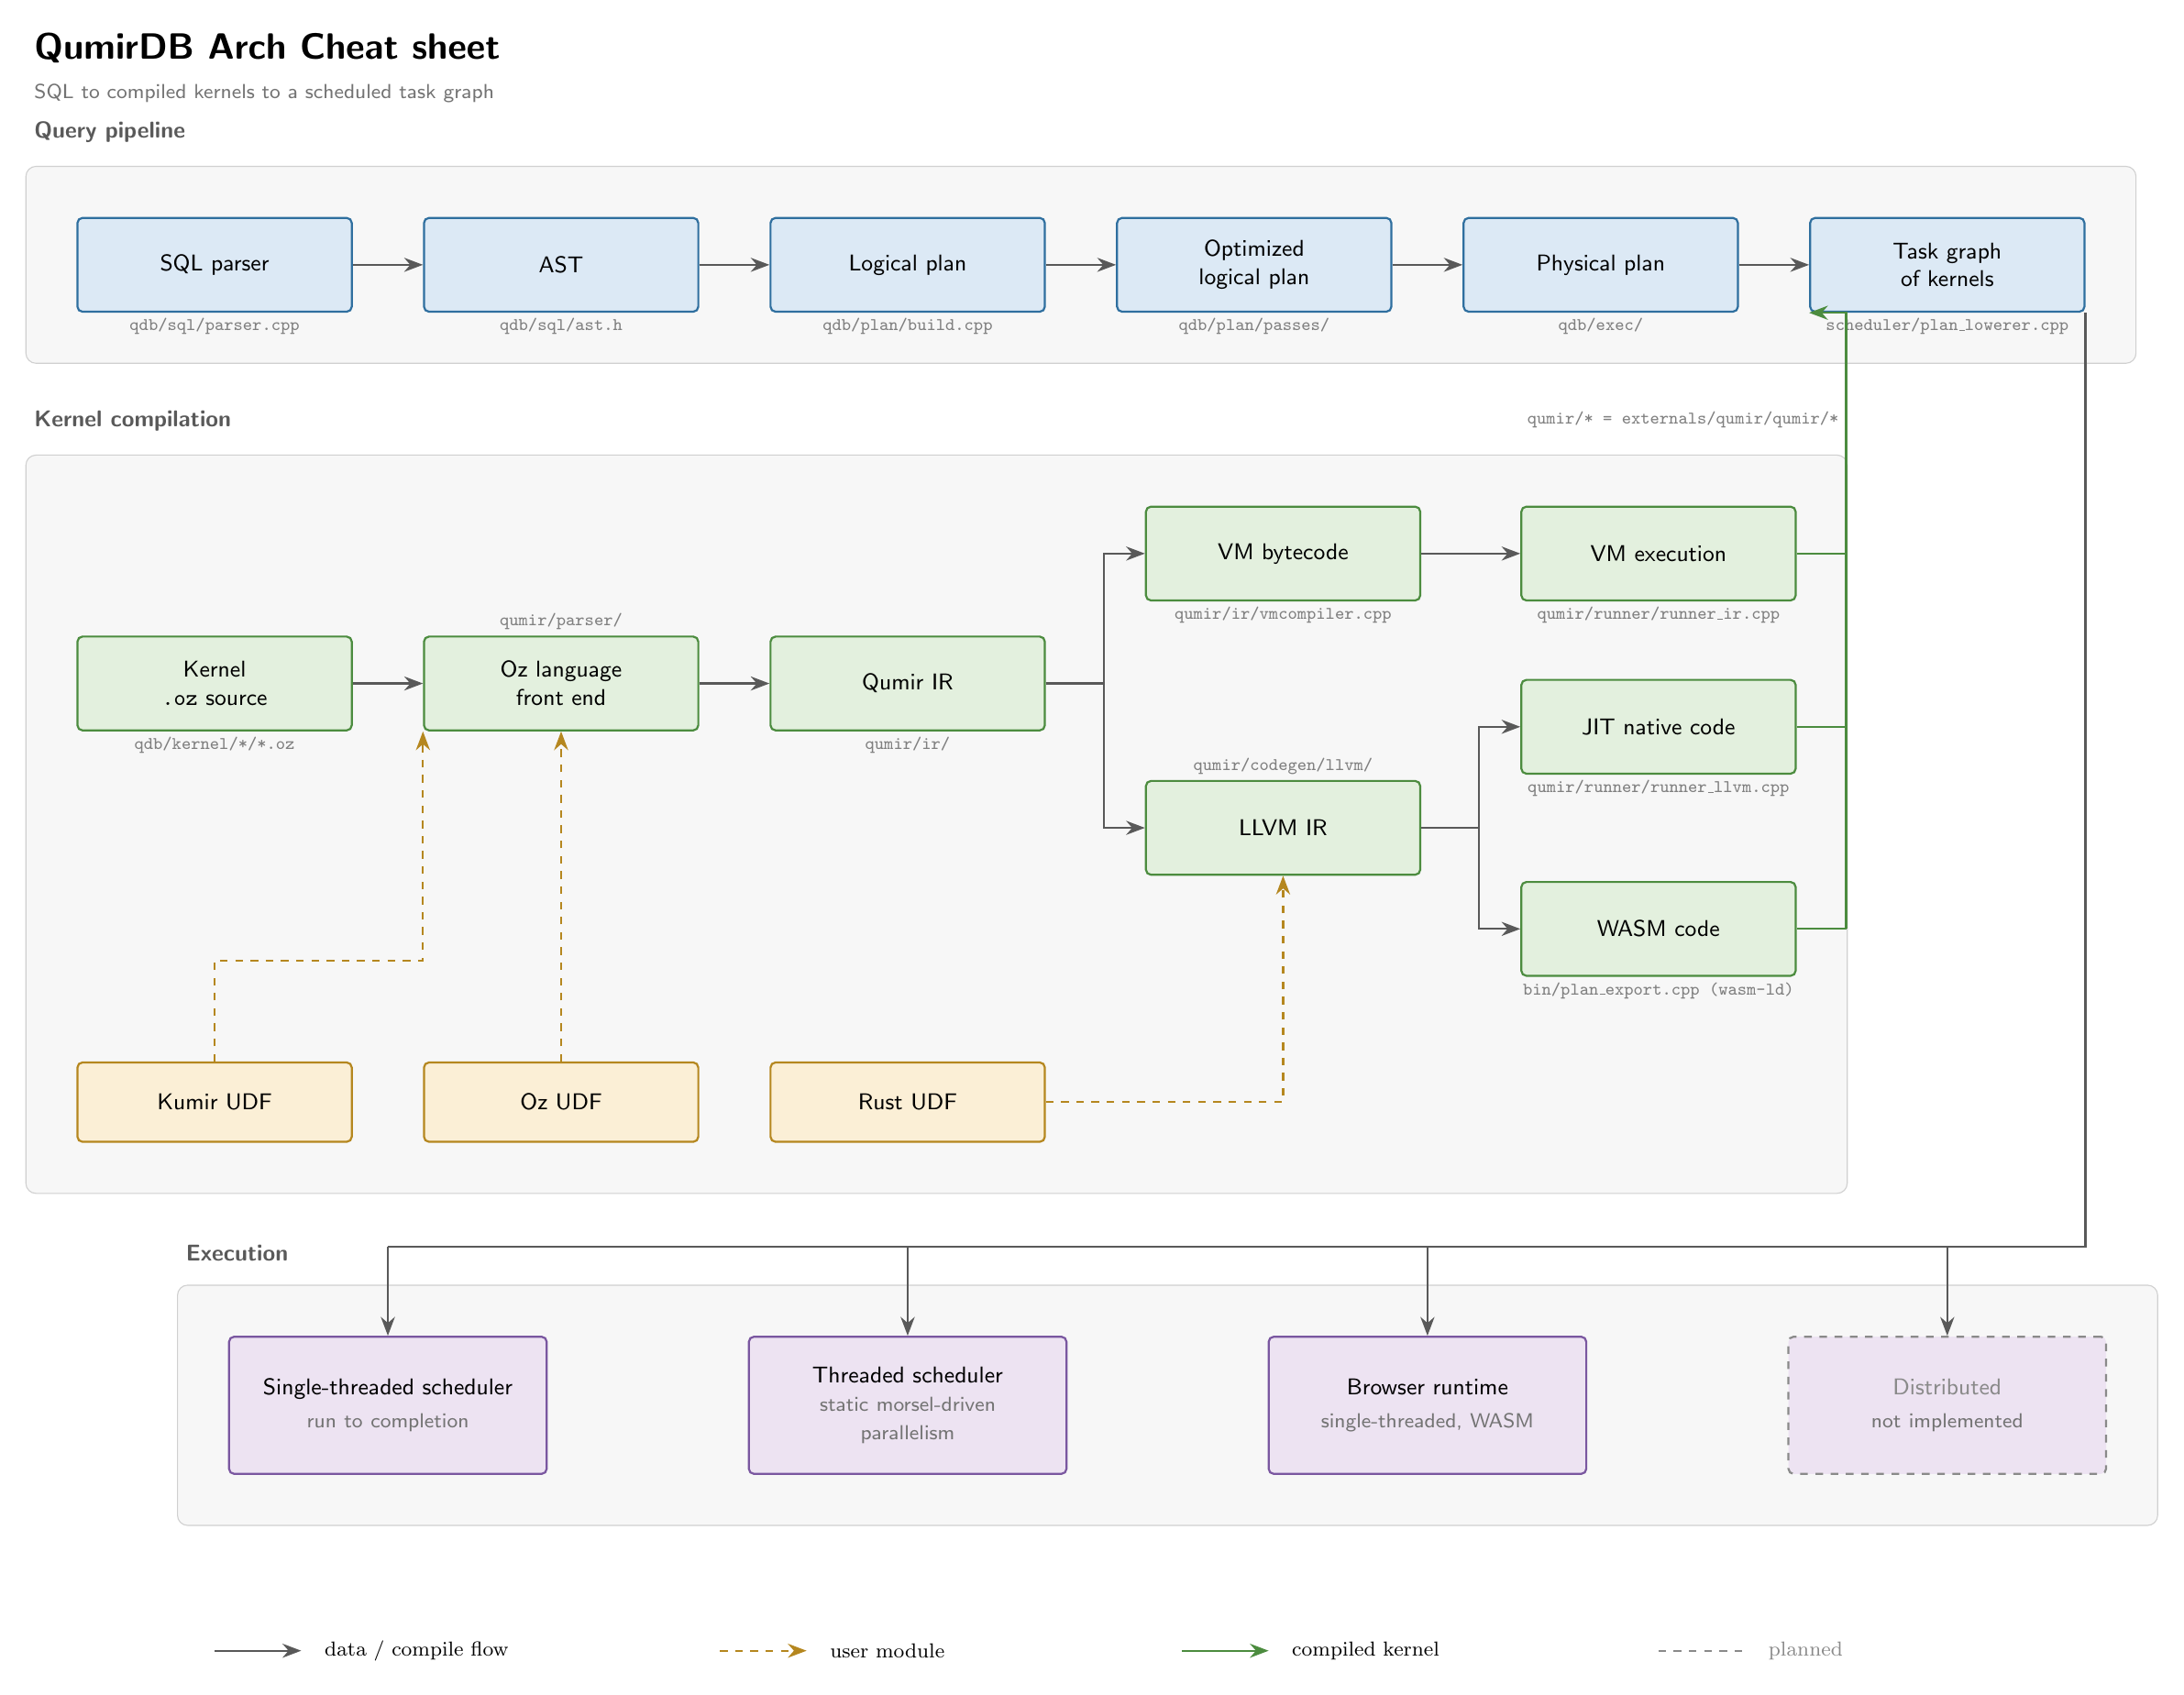
\begin{tikzpicture}[
  x=1mm, y=1mm,
  font=\sffamily\small,
  box/.style={
    rounded corners=2pt, draw, thick, align=center,
    minimum height=13mm, text width=34mm, inner sep=2mm},
  plan/.style={box, fill=planfill, draw=plandraw},
  kernel/.style={box, fill=kernelfill, draw=kerneldraw},
  udf/.style={box, fill=udffill, draw=udfdraw, minimum height=11mm},
  run/.style={box, fill=runfill, draw=rundraw,
              text width=40mm, minimum height=19mm},
  planned/.style={run, dashed, draw=muted, text=muted},
  hint/.style={font=\scriptsize\ttfamily, text=black!50, anchor=north,
               inner sep=0.7mm},
  % Above the box where an incoming arrow needs the space below it.
  hintabove/.style={hint, anchor=south},
  flow/.style={-{Stealth[length=2.6mm]}, thick, draw=black!65},
  feed/.style={flow, draw=udfdraw, dashed},
  link/.style={thick, draw=kerneldraw},
  linkarrow/.style={flow, draw=kerneldraw},
  bus/.style={thick, draw=black!65},
  band/.style={rounded corners=4pt, fill=bandfill, draw=banddraw},
  bandlabel/.style={font=\sffamily\bfseries\small, text=black!65,
                    anchor=south west},
]

%% ------------------------------------------------------------- query pipeline
\node[plan] (parser)    at (  0, 0) {SQL parser};
\node[plan] (ast)       at ( 48, 0) {AST};
\node[plan] (logical)   at ( 96, 0) {Logical plan};
\node[plan] (optimized) at (144, 0) {Optimized\\logical plan};
\node[plan] (physical)  at (192, 0) {Physical plan};
\node[plan] (graph)     at (240, 0) {Task graph\\of kernels};

\foreach \a/\b in {parser/ast, ast/logical, logical/optimized,
                   optimized/physical, physical/graph}
  \draw[flow] (\a) -- (\b);

\node[hint] at (parser.south)    {qdb/sql/parser.cpp};
\node[hint] at (ast.south)       {qdb/sql/ast.h};
\node[hint] at (logical.south)   {qdb/plan/build.cpp};
\node[hint] at (optimized.south) {qdb/plan/passes/};
\node[hint] at (physical.south)  {qdb/exec/};
\node[hint] at (graph.south)     {scheduler/plan\_lowerer.cpp};

%% --------------------------------------------------------- kernel compilation
\node[kernel] (ksrc)   at (  0, -58) {Kernel\\\texttt{.oz} source};
\node[kernel] (oz)     at ( 48, -58) {Oz language\\front end};
\node[kernel] (ir)     at ( 96, -58) {Qumir IR};
\node[kernel] (vmcode) at (148, -40) {VM bytecode};
\node[kernel] (vmexec) at (200, -40) {VM execution};
\node[kernel] (llvm)   at (148, -78) {LLVM IR};
\node[kernel] (jit)    at (200, -64) {JIT native code};
\node[kernel] (wasm)   at (200, -92) {WASM code};

\draw[flow] (ksrc) -- (oz);
\draw[flow] (oz)   -- (ir);
\draw[flow] (ir.east) -- ++(8,0) |- (vmcode.west);
\draw[flow] (ir.east) -- ++(8,0) |- (llvm.west);
\draw[flow] (vmcode) -- (vmexec);
\draw[flow] (llvm.east) -- ++(8,0) |- (jit.west);
\draw[flow] (llvm.east) -- ++(8,0) |- (wasm.west);

\node[hint] at (ksrc.south)   {qdb/kernel/*/*.oz};
\node[hintabove] at (oz.north) {qumir/parser/};
\node[hint] at (ir.south)     {qumir/ir/};
\node[hint] at (vmcode.south) {qumir/ir/vmcompiler.cpp};
\node[hint] at (vmexec.south) {qumir/runner/runner\_ir.cpp};
\node[hint] at (jit.south)    {qumir/runner/runner\_llvm.cpp};
\node[hintabove] at (llvm.north) {qumir/codegen/llvm/};
\node[hint] at (wasm.south)   {bin/plan\_export.cpp (wasm-ld)};

%% --------------------------------------------------------------- user modules
\node[udf] (kumirudf) at (  0, -116) {Kumir UDF};
\node[udf] (ozudf)    at ( 48, -116) {Oz UDF};
\node[udf] (rustudf)  at ( 96, -116) {Rust UDF};

\draw[feed] (kumirudf.north) -- ++(0,14) -| (oz.south west);
\draw[feed] (ozudf.north) -- (oz.south);
\draw[feed] (rustudf.east) -| (llvm.south);

%% ----------------------------------------------------- kernels join the graph
\draw[link] (vmexec.east) -- (226, -40);
\draw[link] (jit.east)    -- (226, -64);
\draw[link] (wasm.east)   -- (226, -92);
\draw[link] (226, -92) -- (226, -40);
\draw[linkarrow] (226, -40) |- (graph.south west);

%% ------------------------------------------------------------------ execution
\node[run] (single) at ( 24, -158)
  {Single-threaded scheduler\sub{run to completion}};
\node[run] (threaded) at ( 96, -158)
  {Threaded scheduler\sub{static morsel-driven\\parallelism}};
\node[run] (browser) at (168, -158)
  {Browser runtime\sub{single-threaded, WASM}};
\node[planned] (distrib) at (240, -158)
  {Distributed\sub{not implemented}};

\draw[bus] (graph.south east) |- (24, -136);
\foreach \n in {single, threaded, browser, distrib}
  \draw[flow] (\n.north |- 0,-136) -- (\n.north);

%% ---------------------------------------------------------------------- bands
\begin{scope}[on background layer]
  \node[band, fit=(parser)(graph), inner sep=7mm] (band1) {};
  \node[band, fit=(ksrc)(vmcode)(vmexec)(wasm)(rustudf), inner sep=7mm]
    (band2) {};
  \node[band, fit=(single)(distrib), inner sep=7mm] (band3) {};
\end{scope}

\node[bandlabel] at ([yshift=2mm]band1.north west) {Query pipeline};
\node[bandlabel] at ([yshift=2mm]band2.north west) {Kernel compilation};
\node[anchor=south east, font=\scriptsize\ttfamily, text=black!50]
  at ([yshift=2.5mm]band2.north east) {qumir/* = externals/qumir/qumir/*};
\node[bandlabel] at ([yshift=2mm]band3.north west) {Execution};

%% ---------------------------------------------------------------------- title
\node[anchor=south west, font=\sffamily\bfseries\Large]
  (title) at ([yshift=13mm]band1.north west) {QumirDB Arch Cheat sheet};
\node[anchor=north west, font=\sffamily\footnotesize, text=black!55]
  at ([yshift=-0.5mm]title.south west)
  {SQL to compiled kernels to a scheduled task graph};

%% --------------------------------------------------------------------- legend
\begin{scope}[shift={(0,-192)}]
  \draw[flow]      (0,0)  -- (12,0);  \node[anchor=west, font=\footnotesize]
    at (14,0) {data / compile flow};
  \draw[feed]      (70,0) -- (82,0);  \node[anchor=west, font=\footnotesize]
    at (84,0) {user module};
  \draw[linkarrow] (134,0) -- (146,0); \node[anchor=west, font=\footnotesize]
    at (148,0) {compiled kernel};
  \draw[dashed, thick, draw=muted] (200,0) -- (212,0);
  \node[anchor=west, font=\footnotesize, text=muted] at (214,0) {planned};
\end{scope}

\end{tikzpicture}
\end{document}
